% Options for packages loaded elsewhere
\PassOptionsToPackage{unicode}{hyperref}
\PassOptionsToPackage{hyphens}{url}
%
\documentclass[
  man]{apa6}
\usepackage{amsmath,amssymb}
\usepackage{iftex}
\ifPDFTeX
  \usepackage[T1]{fontenc}
  \usepackage[utf8]{inputenc}
  \usepackage{textcomp} % provide euro and other symbols
\else % if luatex or xetex
  \usepackage{unicode-math} % this also loads fontspec
  \defaultfontfeatures{Scale=MatchLowercase}
  \defaultfontfeatures[\rmfamily]{Ligatures=TeX,Scale=1}
\fi
\usepackage{lmodern}
\ifPDFTeX\else
  % xetex/luatex font selection
\fi
% Use upquote if available, for straight quotes in verbatim environments
\IfFileExists{upquote.sty}{\usepackage{upquote}}{}
\IfFileExists{microtype.sty}{% use microtype if available
  \usepackage[]{microtype}
  \UseMicrotypeSet[protrusion]{basicmath} % disable protrusion for tt fonts
}{}
\makeatletter
\@ifundefined{KOMAClassName}{% if non-KOMA class
  \IfFileExists{parskip.sty}{%
    \usepackage{parskip}
  }{% else
    \setlength{\parindent}{0pt}
    \setlength{\parskip}{6pt plus 2pt minus 1pt}}
}{% if KOMA class
  \KOMAoptions{parskip=half}}
\makeatother
\usepackage{xcolor}
\usepackage{graphicx}
\makeatletter
\def\maxwidth{\ifdim\Gin@nat@width>\linewidth\linewidth\else\Gin@nat@width\fi}
\def\maxheight{\ifdim\Gin@nat@height>\textheight\textheight\else\Gin@nat@height\fi}
\makeatother
% Scale images if necessary, so that they will not overflow the page
% margins by default, and it is still possible to overwrite the defaults
% using explicit options in \includegraphics[width, height, ...]{}
\setkeys{Gin}{width=\maxwidth,height=\maxheight,keepaspectratio}
% Set default figure placement to htbp
\makeatletter
\def\fps@figure{htbp}
\makeatother
\setlength{\emergencystretch}{3em} % prevent overfull lines
\providecommand{\tightlist}{%
  \setlength{\itemsep}{0pt}\setlength{\parskip}{0pt}}
\setcounter{secnumdepth}{-\maxdimen} % remove section numbering
% Make \paragraph and \subparagraph free-standing
\ifx\paragraph\undefined\else
  \let\oldparagraph\paragraph
  \renewcommand{\paragraph}[1]{\oldparagraph{#1}\mbox{}}
\fi
\ifx\subparagraph\undefined\else
  \let\oldsubparagraph\subparagraph
  \renewcommand{\subparagraph}[1]{\oldsubparagraph{#1}\mbox{}}
\fi
\ifLuaTeX
\usepackage[bidi=basic]{babel}
\else
\usepackage[bidi=default]{babel}
\fi
\babelprovide[main,import]{english}
% get rid of language-specific shorthands (see #6817):
\let\LanguageShortHands\languageshorthands
\def\languageshorthands#1{}
% Manuscript styling
\usepackage{upgreek}
\captionsetup{font=singlespacing,justification=justified}

% Table formatting
\usepackage{longtable}
\usepackage{lscape}
% \usepackage[counterclockwise]{rotating}   % Landscape page setup for large tables
\usepackage{multirow}		% Table styling
\usepackage{tabularx}		% Control Column width
\usepackage[flushleft]{threeparttable}	% Allows for three part tables with a specified notes section
\usepackage{threeparttablex}            % Lets threeparttable work with longtable

% Create new environments so endfloat can handle them
% \newenvironment{ltable}
%   {\begin{landscape}\centering\begin{threeparttable}}
%   {\end{threeparttable}\end{landscape}}
\newenvironment{lltable}{\begin{landscape}\centering\begin{ThreePartTable}}{\end{ThreePartTable}\end{landscape}}

% Enables adjusting longtable caption width to table width
% Solution found at http://golatex.de/longtable-mit-caption-so-breit-wie-die-tabelle-t15767.html
\makeatletter
\newcommand\LastLTentrywidth{1em}
\newlength\longtablewidth
\setlength{\longtablewidth}{1in}
\newcommand{\getlongtablewidth}{\begingroup \ifcsname LT@\roman{LT@tables}\endcsname \global\longtablewidth=0pt \renewcommand{\LT@entry}[2]{\global\advance\longtablewidth by ##2\relax\gdef\LastLTentrywidth{##2}}\@nameuse{LT@\roman{LT@tables}} \fi \endgroup}

% \setlength{\parindent}{0.5in}
% \setlength{\parskip}{0pt plus 0pt minus 0pt}

% Overwrite redefinition of paragraph and subparagraph by the default LaTeX template
% See https://github.com/crsh/papaja/issues/292
\makeatletter
\renewcommand{\paragraph}{\@startsection{paragraph}{4}{\parindent}%
  {0\baselineskip \@plus 0.2ex \@minus 0.2ex}%
  {-1em}%
  {\normalfont\normalsize\bfseries\itshape\typesectitle}}

\renewcommand{\subparagraph}[1]{\@startsection{subparagraph}{5}{1em}%
  {0\baselineskip \@plus 0.2ex \@minus 0.2ex}%
  {-\z@\relax}%
  {\normalfont\normalsize\itshape\hspace{\parindent}{#1}\textit{\addperi}}{\relax}}
\makeatother

% \usepackage{etoolbox}
\makeatletter
\patchcmd{\HyOrg@maketitle}
  {\section{\normalfont\normalsize\abstractname}}
  {\section*{\normalfont\normalsize\abstractname}}
  {}{\typeout{Failed to patch abstract.}}
\patchcmd{\HyOrg@maketitle}
  {\section{\protect\normalfont{\@title}}}
  {\section*{\protect\normalfont{\@title}}}
  {}{\typeout{Failed to patch title.}}
\makeatother

\usepackage{xpatch}
\makeatletter
\xapptocmd\appendix
  {\xapptocmd\section
    {\addcontentsline{toc}{section}{\appendixname\ifoneappendix\else~\theappendix\fi\\: #1}}
    {}{\InnerPatchFailed}%
  }
{}{\PatchFailed}
\keywords{keywords\newline\indent Word count: X}
\DeclareDelayedFloatFlavor{ThreePartTable}{table}
\DeclareDelayedFloatFlavor{lltable}{table}
\DeclareDelayedFloatFlavor*{longtable}{table}
\makeatletter
\renewcommand{\efloat@iwrite}[1]{\immediate\expandafter\protected@write\csname efloat@post#1\endcsname{}}
\makeatother
\usepackage{lineno}

\linenumbers
\usepackage{csquotes}
\ifLuaTeX
  \usepackage{selnolig}  % disable illegal ligatures
\fi
\IfFileExists{bookmark.sty}{\usepackage{bookmark}}{\usepackage{hyperref}}
\IfFileExists{xurl.sty}{\usepackage{xurl}}{} % add URL line breaks if available
\urlstyle{same}
\hypersetup{
  pdftitle={The title},
  pdfauthor={First Author1 \& Ernst-August Doelle1,2},
  pdflang={en-EN},
  pdfkeywords={keywords},
  hidelinks,
  pdfcreator={LaTeX via pandoc}}

\title{The title}
\author{First Author\textsuperscript{1} \& Ernst-August Doelle\textsuperscript{1,2}}
\date{}


\shorttitle{Title}

\authornote{

Add complete departmental affiliations for each author here. Each new line herein must be indented, like this line.

Enter author note here.

The authors made the following contributions. First Author: Conceptualization, Writing - Original Draft Preparation, Writing - Review \& Editing; Ernst-August Doelle: Writing - Review \& Editing, Supervision.

Correspondence concerning this article should be addressed to First Author, Postal address. E-mail: \href{mailto:my@email.com}{\nolinkurl{my@email.com}}

}

\affiliation{\vspace{0.5cm}\textsuperscript{1} Wilhelm-Wundt-University\\\textsuperscript{2} Konstanz Business School}

\abstract{%
One or two sentences providing a \textbf{basic introduction} to the field, comprehensible to a scientist in any discipline.
}



\begin{document}
\maketitle

\hypertarget{results}{%
\section{Results}\label{results}}

The aggregated data-set describes 316,835 observations of daily physical activity and sleep from 24,935 unique participants. Table \ref{demo} shows demographic information. A table of study characteristics can be found in supplementary materials.

\hypertarget{the-effects-of-physical-activity-volume-on-sleep}{%
\subsection{The effects of physical activity volume on sleep}\label{the-effects-of-physical-activity-volume-on-sleep}}

We explored the effects of physical activity on sleep (RQ1) using mixed-effects models. We estimated the effect of physical activity volume on sleep by age, and the results are presented in Table \ref{tab:sleep-by-volume} and Figure \ref{fig:sleep-by-volume-fig}. There was no meaningful relationship between physical activity volume and sleep duration. However, a positive curvilinear relationship was observed between physical activity volume and sleep efficiency, onset, and regularity, which interacted with age. Sleep efficiency improved with greater physical activity volume, but improvements tapered off for older individuals. Physical activity volume and sleep onset had a positive association for younger individuals, but a negative association for older individuals, where sleep onset was reduced among those with the highest physical activity. There was a strong positive association between physical activity volume and sleep regularity, which was strongest among older participants. For participants aged 35 years and above, this link weakened among those with a physical activity volume greater than two standard deviations.

\renewcommand{\arraystretch}{0.7}

\begin{table}[tbp]

\begin{center}
\begin{threeparttable}

\caption{\label{tab:sleep-by-volume}Sleep on physical activity volume controlling for SES, gender and BMI}

\begin{tabular}{lllll}
\toprule
Term & \multicolumn{1}{c}{$\beta$ [95\% CI]} & \multicolumn{1}{c}{SE} & \multicolumn{1}{c}{t} & \multicolumn{1}{c}{p}\\
\midrule
Sleep duration &  &  &  & \\
\ \ \ (Intercept) & -0.37 [-0.94, 0.20] & 0.29 & -1.28 & .291\\
\ \ \ Scale  pa  volume & 0.03 [0.00, 0.07] & 0.02 & 1.96 & .050\\
\ \ \ Age & 0.00 [-0.01, 0.00] & 0.00 & -0.29 & .797\\
\ \ \ Scale  pa  volume$^2$ & 0.00 [-0.01, 0.01] & 0.00 & 0.11 & .912\\
\ \ \ Scale  pa  volume:age & 0.00 [0.00, 0.00] & 0.00 & 0.92 & .359\\
\ \ \ Age:scale  pa  volume$^2$ & 0.00 [0.00, 0.00] & 0.00 & -0.94 & .349\\
Sleep efficiency &  &  &  & \\
\ \ \ (Intercept) & -0.90 [-1.29, -0.50] & 0.20 & -4.46 & .001\\
\ \ \ Scale  pa  volume & 0.23 [0.20, 0.27] & 0.02 & 12.97 & < .001\\
\ \ \ Age & 0.01 [0.01, 0.01] & 0.00 & 9.99 & .002\\
\ \ \ Scale  pa  volume$^2$ & -0.02 [-0.03, -0.01] & 0.00 & -4.77 & < .001\\
\ \ \ Scale  pa  volume:age & 0.00 [0.00, 0.00] & 0.00 & -5.16 & < .001\\
\ \ \ Age:scale  pa  volume$^2$ & 0.00 [0.00, 0.00] & 0.00 & -0.50 & .617\\
Sleep onset &  &  &  & \\
\ \ \ (Intercept) & -0.98 [-1.50, -0.47] & 0.26 & -3.77 & .060\\
\ \ \ Scale  pa  volume & 0.11 [0.09, 0.14] & 0.01 & 8.32 & < .001\\
\ \ \ Age & 0.02 [0.02, 0.02] & 0.00 & 9.81 & .007\\
\ \ \ Scale  pa  volume$^2$ & -0.01 [-0.02, -0.01] & 0.00 & -4.73 & < .001\\
\ \ \ Scale  pa  volume:age & 0.00 [0.00, 0.00] & 0.00 & -8.70 & < .001\\
\ \ \ Age:scale  pa  volume$^2$ & 0.00 [0.00, 0.00] & 0.00 & 2.34 & .034\\
Sleep regularity &  &  &  & \\
\ \ \ (Intercept) & -0.13 [-0.39, 0.13] & 0.13 & -0.96 & .415\\
\ \ \ Scale  pa  volume & 0.33 [0.29, 0.36] & 0.02 & 19.10 & < .001\\
\ \ \ Age & 0.01 [0.00, 0.01] & 0.00 & 5.07 & .019\\
\ \ \ Scale  pa  volume$^2$ & -0.03 [-0.03, -0.02] & 0.00 & -5.74 & < .001\\
\ \ \ Scale  pa  volume:age & 0.00 [0.00, 0.00] & 0.00 & 0.64 & .540\\
\ \ \ Age:scale  pa  volume$^2$ & 0.00 [0.00, 0.00] & 0.00 & -3.33 & .006\\
\bottomrule
\addlinespace
\end{tabular}

\begin{tablenotes}[para]
\normalsize{\textit{Note.} Adjusted for SES, BMI, and sex. }
\end{tablenotes}

\end{threeparttable}
\end{center}

\end{table}

\begin{figure}
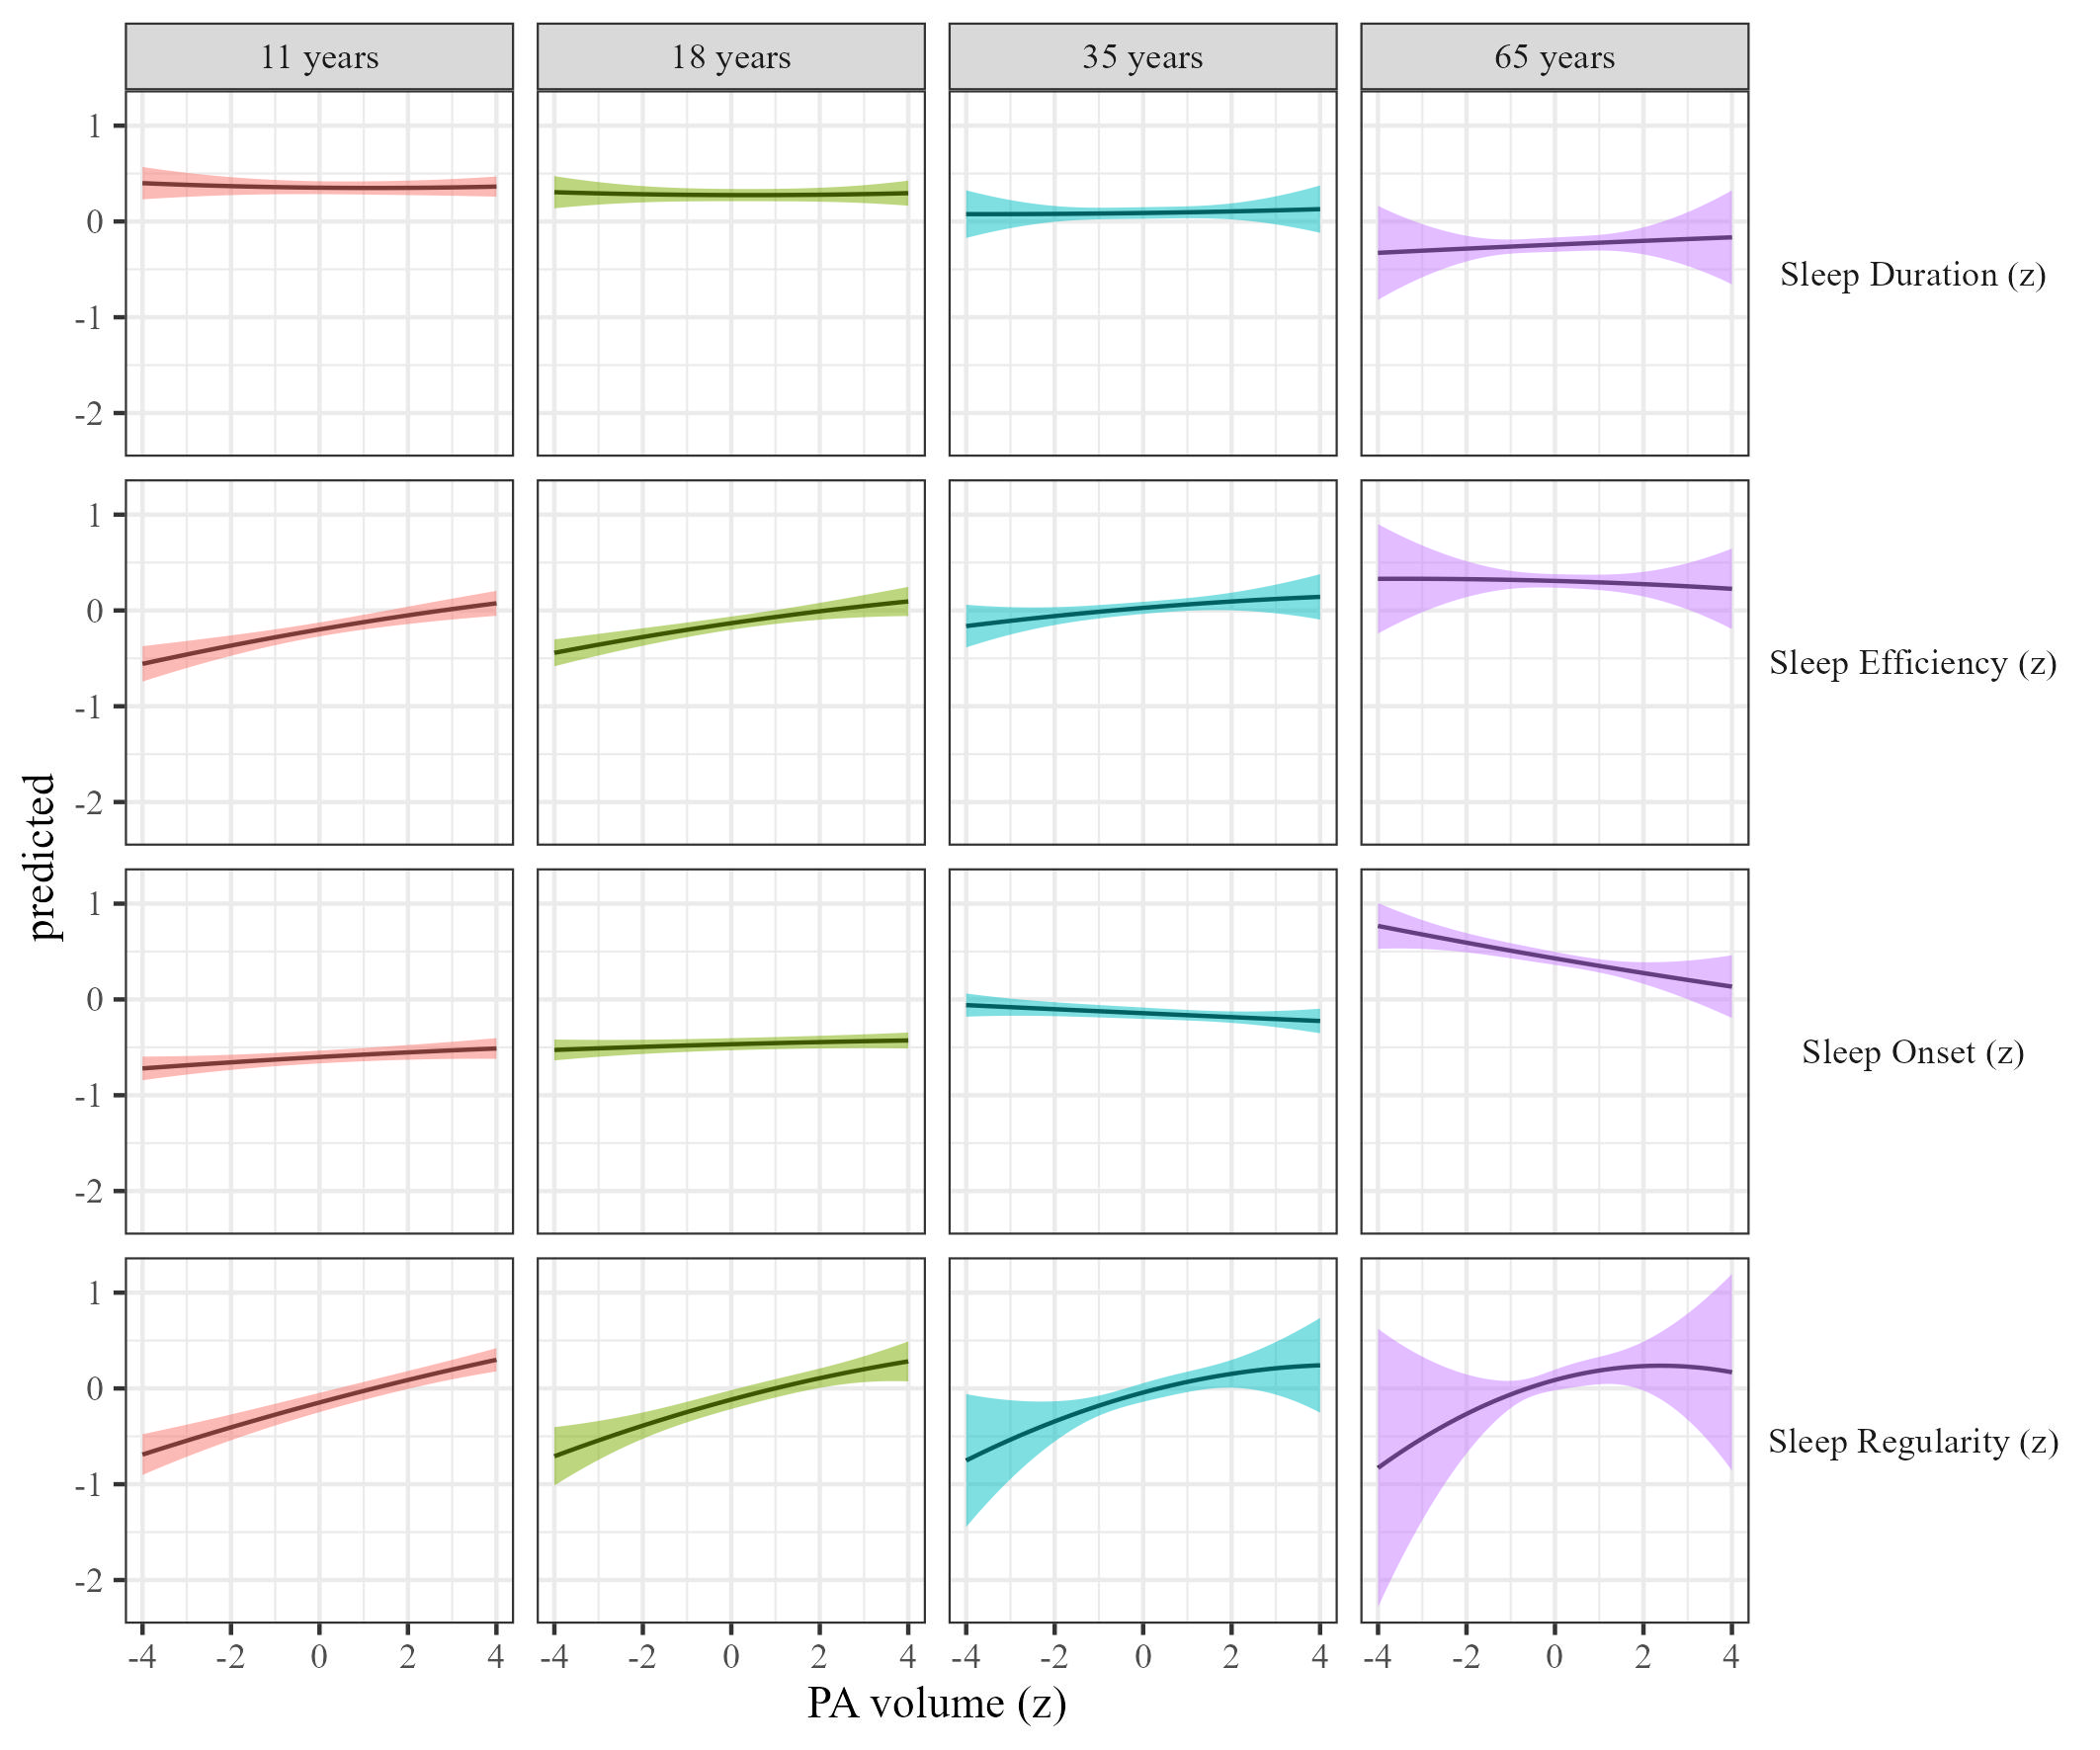
\includegraphics[width=7.08in]{../Figures/sleep on pa_volume} \caption{Sleep metrics on Physical activity volume}\label{fig:sleep-by-volume-fig}
\end{figure}


\end{document}
